\clearpage 
\newpage

%\section*{Figure legends}

\begin{figure}
  \centering
  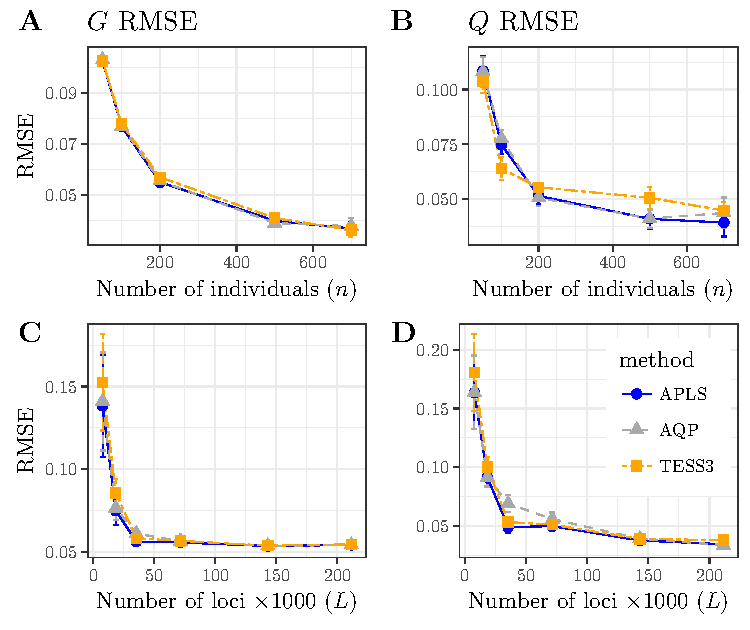
\includegraphics[width=\textwidth]{./Figures/figure1.pdf}
  \caption{{\bf Root Mean Squared Errors (RMSEs) for the $Q$ and $G$ matrix
      estimates}. Simulations of spatially admixed populations. A-B) Statistical
    errors for APLS, AQP and {\tt tess3} estimates as a function of the sample
    size, $n$ ($L \sim 10^4$). C-D) Statistical errors for APLS, AQP and {\tt
      tess3} estimates as a function of the number of loci, $L$ ($n = 200$).}
  \label{fig:fig1}
\end{figure}  

\clearpage 
\newpage

\begin{figure}
  \centering
  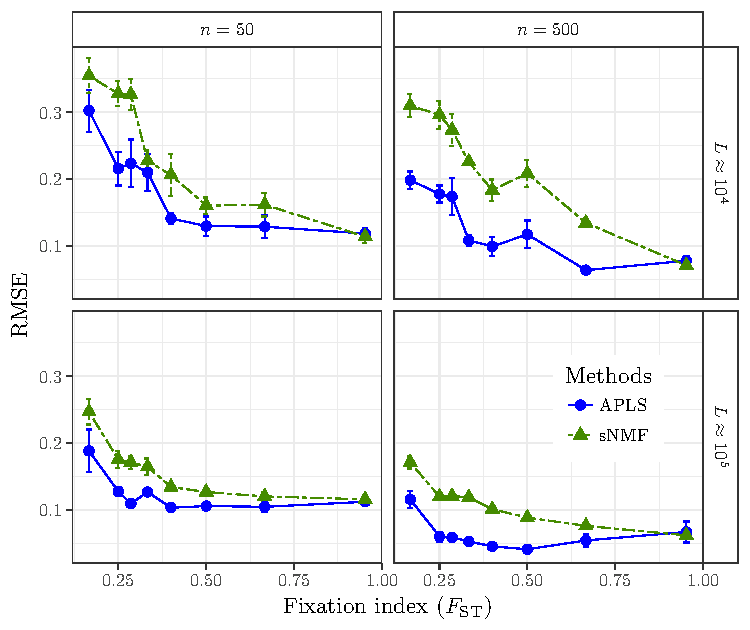
\includegraphics[width=\textwidth]{./Figures/figure2.pdf}
  \caption{{\bf Root Mean Squared Errors (RMSEs) for the $Q$ estimates.}
    Simulations of spatially admixed populations for several values of fixation
    index ($F_{\rm ST}$) between ancestral populations. Ancestral populations
    are simulated with Wright's two-island models and the fixation index is
    defined as $1 / (1 + 4 N_0 m)$ where $m$ is the migration rate and $N_0$ the
    effective population size. The statistical errors for sNMF and APLS are
    represented as a function of $F_{\rm ST}$. }
  \label{fig:fig2}
\end{figure}  

\clearpage 
\newpage

\begin{figure}
  \centering
  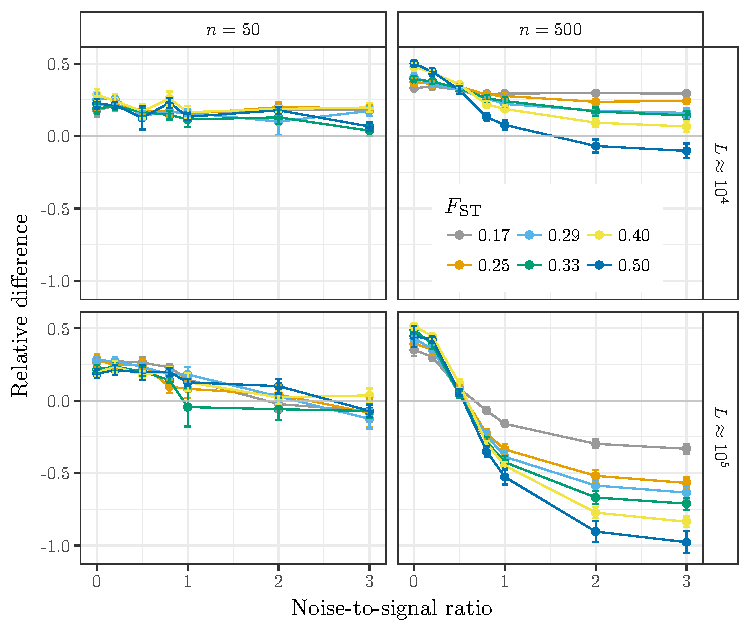
\includegraphics[width=\textwidth]{./Figures/figure2_5.pdf}
  \caption{{\bf Relative differences RMSE for APLS and {\tt snmf} estimates}}
  \label{fig:fig2_5}
\end{figure}  

\clearpage 
\newpage



\begin{figure}
  \centering
  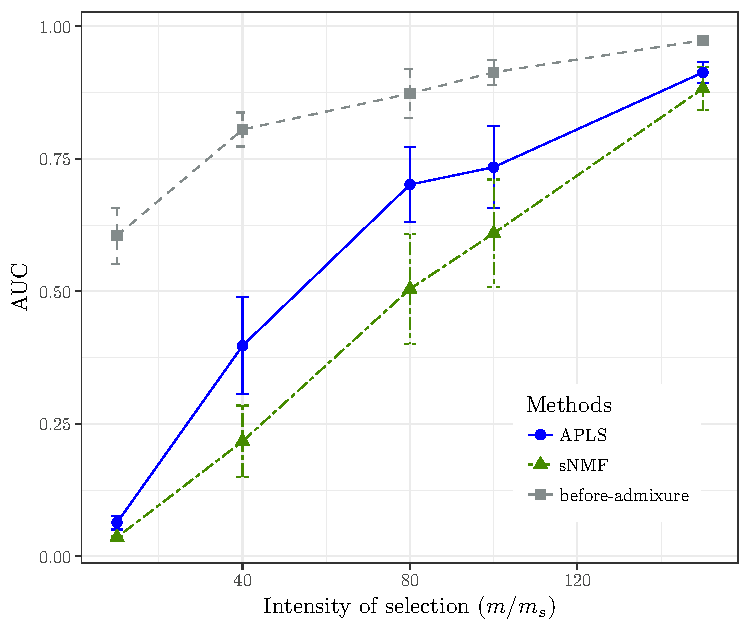
\includegraphics[width=\textwidth]{./Figures/figure3.pdf}
  \caption{ {\bf Area under the precision-recall curve (AUC)}. Neutrality tests
    applied to simulations of spatially admixed populations. AUCs for tests
    based on $F_{\rm ST}$ with the true ancestral populations, spatial ancestry
    estimates computed with APLS algorithms, non-spatial ({\tt structure}-like)
    ancestry estimates computed with the {\tt snmf} algorithm. The relative
    intensity of selection in ancestral populations, defined as the ratio
    $m/m_s$, was varied in the range $1-160$.}
  \label{fig:fig3}
\end{figure}


\clearpage 
\newpage

\begin{figure}
  \centering
  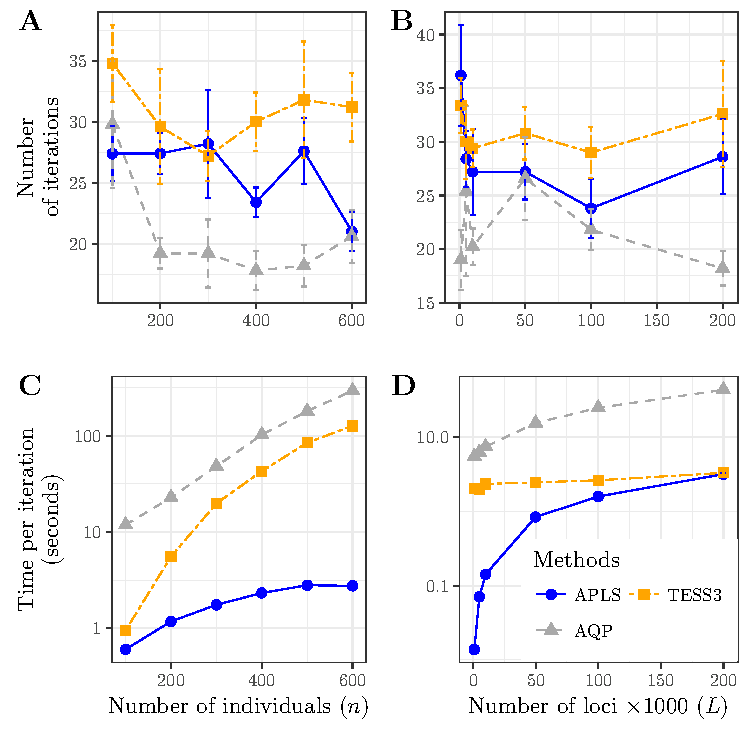
\includegraphics[width=\textwidth]{./Figures/figure4.pdf}
  \caption{{\bf Number of iterations and runtimes for the AQP, APLS and {\tt
        tess3} algorithm implementations}. A-B) Total number of iterations
    before an algorithm reached a steady solution. C-D) Runtime for a single
    iteration (seconds). The number of SNPs was kept fixed to $L = 50$k in A and
    C. The number of individuals was kept fixed to $n = 150$ in B and D.}
  \label{fig:fig4}
\end{figure}

\clearpage 
\newpage

\begin{figure}
  \centering
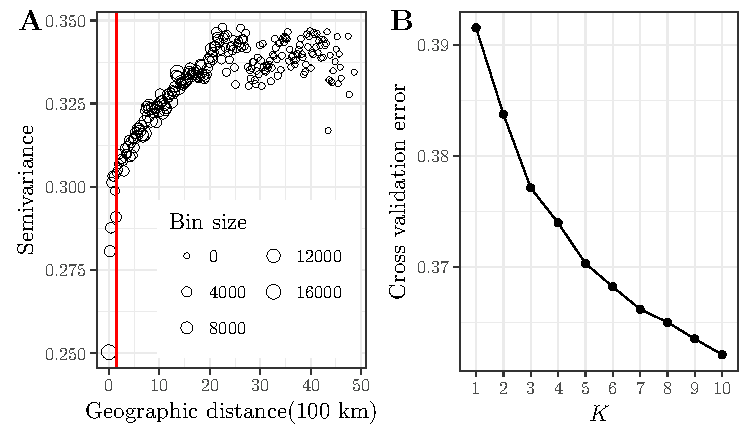
\includegraphics[width=\textwidth]{./Figures/figure5.pdf}
\caption{{\bf Range $\sigma$ and choice of $K$ for the APLS algorithm}. A)
  Empirical variogram for the {\it A. thaliana} data. The red vertical line
  shows the range value $\sigma = 1.5$. B) Cross validation error as function of
  the number of ancestral populations, $K$.}
  \label{fig:fig5}
\end{figure}

\clearpage 
\newpage

\begin{figure}
  \centering
  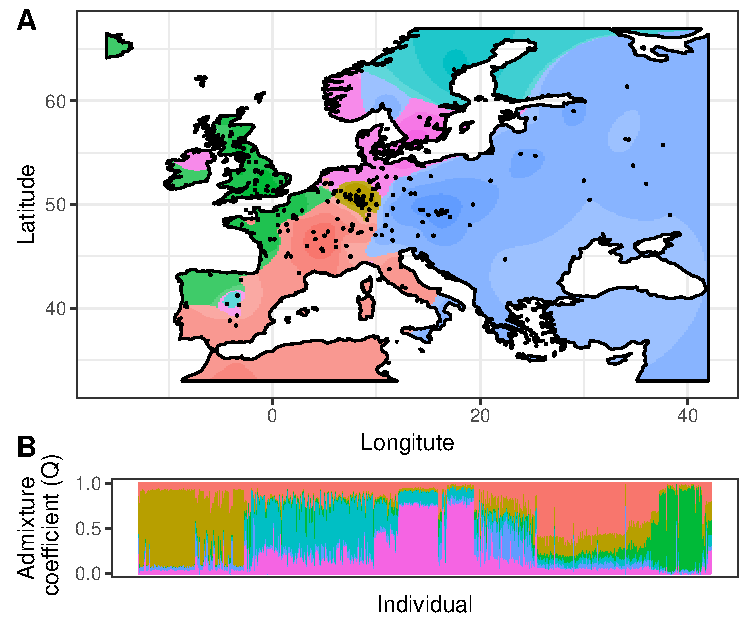
\includegraphics[width=\textwidth]{./Figures/map.pdf}
  \caption{{\bf {\it A. thaliana} ancestry coeficients}. Ancestry coefficient
    estimates computed by the APLS algorithm with $K=6$ ancestral populations
    and $\sigma = 1.5$ for the range parameter. A) Geographic map of ancestry
    coefficients. B) Barplot of ancestry coefficients.}
  \label{fig:map}
\end{figure}

\clearpage 
\newpage

\begin{figure}
  \centering
  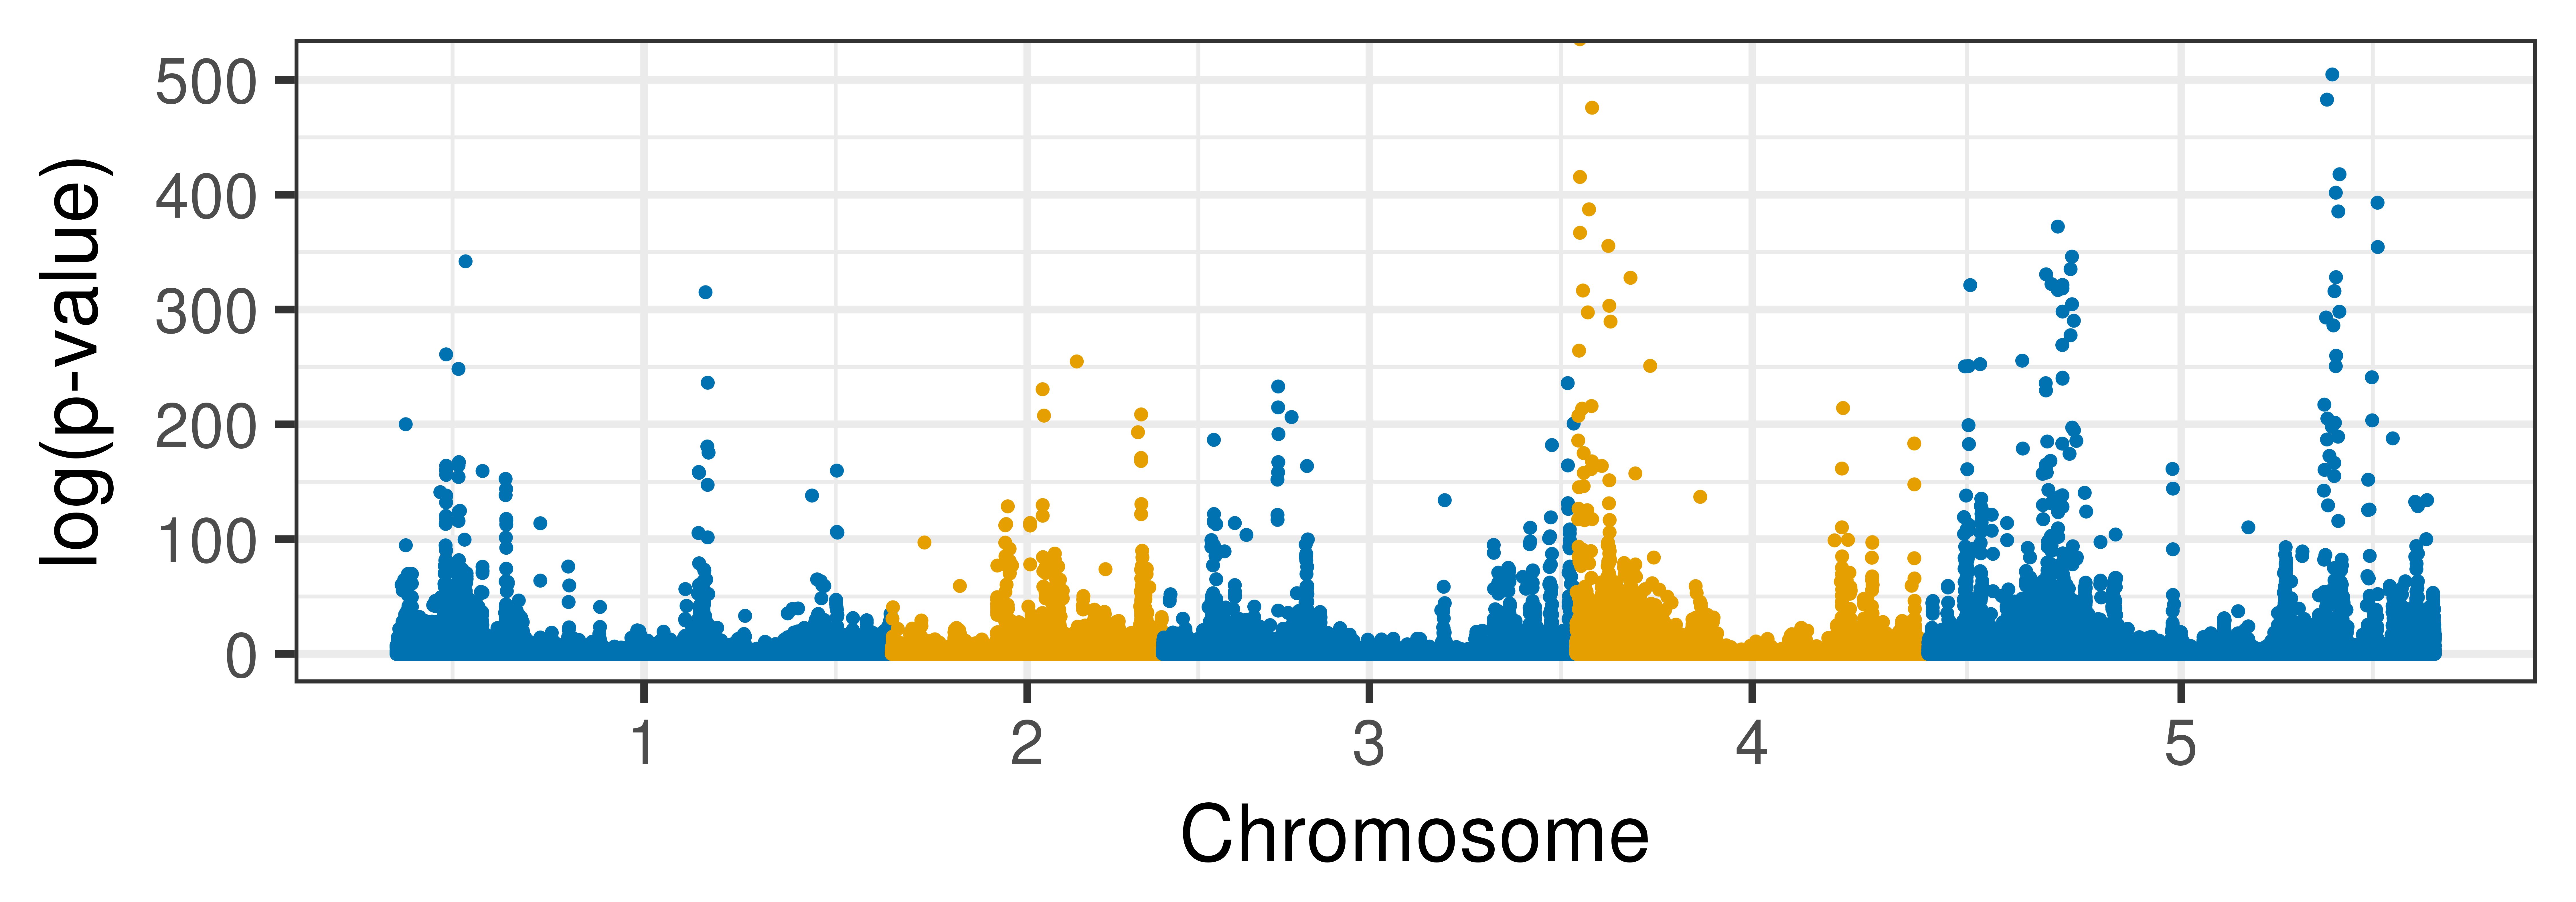
\includegraphics[width=\textwidth]{./Figures/manhattanplot.png}
  % 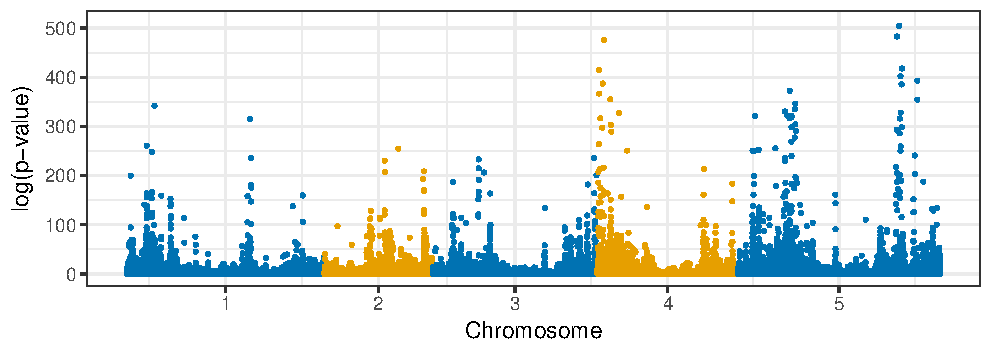
\includegraphics[width=\textwidth]{../Figure5/Figures/manhattanplot.pdf}
  \caption{{\bf Local adaptation in European lines of \bf {\it A. thaliana} }.
    Manhattan plot of $-\log(p$\rm -value$)$. $p$-value were computed from
    population structure estimated by the APLS algorithm with $K=6$ ancestral
    populations and $\sigma = 1.5$ for the range parameter.}
  \label{fig:man}
\end{figure}

\clearpage 
\newpage
